\chapter{Испытание и обоснование эффективности предлагаемых подходов}
\section{Проектирование ПО}
Разработанное программное обеспечение должно соответствовать техническому заданию представленное в Приложении 
А и должна обеспечивать возможность выполнения следующих ниже функций:
\begin{enumerate}
    \item Предоставлять возможность сохранять и загружать данные используемые для работы программы:
    \begin{itemize}
        \item загрузка кластеризованных данных о перемещении;
        \item преобразование загруженных данных во внутренний формат программы;
        \item сохранения расчётных данных для последующей обработки;
    \end{itemize}
    \item Предоставлять возможность по построению матрицы корреспонденций по данным о перемещении для 
        для последующего построения транспортной сети.
    \item Предоставлять возможность анализа графа корреспонденций для выбора узлов отправления-назначения для 
        последующего построения транспортной сети.
    \item Предоставлять функцию построения маршрутной сети по заданным параметрам, включающая следующие 
        пункты:
    \begin{itemize}
        \item инициализации первичной маршрутной сети;
        \item построения маршрутной сети по заданной метрике;
        \item модификация маршрутной сети;
        \item взаимодействие с программных обеспечение OSRM;
    \end{itemize}
    \item Предоставлять возможность производить оценку построенной маршрутной сети, по следующим критериям:
    \begin{itemize}
        \item оценка маршрута по критерию (длина, количество пассажиров и т.~п.);
        \item общая оценка маршрутной сети;
        \item многокритериальная оценка.
    \end{itemize}
\end{enumerate}

Подробности по проектированию ПО описаны в Приложении А. Рассмотренные алгоритмы из главы \ref{chp:methods} 
были реализованы с использованием языка программирования Python и сервиса построения маршрутов Open Source 
Routing Machine (OSRM) для расчёта расстояния между узлами графа по городским дорогам. Программный код 
опубликован на хостинге Github (подробнее в Приложении В).

\section{Методика проведения эксперимента}
Для оценки эффективности алгоритма и изучения его специфики, были проведены эксперименты в ходе которых 
менялось количество узлов в дорожном графе и количество создаваемых маршрутов в городской сети, а также 
несколько вариантов реализации данного метода. Наиболее интересным случаем является, когда обрабатывается 
большое число узлов в графе или большое число геопространственных данных.

Были сгенерированы данных о предпочтениях по перемещению жителей среднего по размерам города с примерным 
числом жителей около \( 350\ 000 \). В качестве результата, было получено \( 6000 \) пар точек 
отправления-назначения или \( 12000 \) точек в общей сложности. Матрица корреспонденций в данном случае имеет 
очень большой размер \( 6000 \times 6000 \) элементов, где элемент с индексом \( i, j \) имеет значение 
\( 0 \) -- отсутствие связи между \( i \)-ой и \( j \)-ой точкой, а \( 1 \) соответственно связь.

Для того, чтобы уменьшить размер матрицы корреспонденций и понять наиболее густонаселённые места, был 
применён алгоритм кластеризации точек отправления-назначения, который не входит в рассмотрение в данной 
работе.

Для того чтобы понять какое количество кластеров (или узлов) влияет на эффективность работы предложенного 
алгоритма было предложено произвести варьирование параметров: количество кластеров и количество маршрутов для 
построения.

Критериями для оценки эффективности разработанных алгоритмов является:
\begin{itemize}
    \item время затраченное на расчёт;
    \item длина полученной маршрутной сети.
\end{itemize}

\chapter{Методология и результаты}
\section{Проведение эксперимента и описание результатов}
По мере того как количество кластеров изменяется получаем различные варианты производительности алгоритма. 
В проводимых экспериментах число узлов изменяется в диапазоне от \( 100 \) до \( 300 \).

Количество маршрутов для построения так же влияет на скорость работы предложенного алгоритма. Очевидно, что 
минимальное количество маршрутов определяется числом пар терминальных маршрутов. В данном случае варьирование 
числа маршрутов было произведено в интервале от \( 8 \) до \( 100 \) в зависимости от количества узлов.

В эксперименте использовалось эмпирическое правило, что число узлов должно быть в \( 20 \) раз больше, чем 
число маршрутов. Для упрощения оценки производительности применяется общая длина сети в качестве критерия 
качества. Поскольку эта оценка производится во внешнем цикле, то она не имеет большого влияния на выполнение 
алгоритма. Кроме того не была использована информация о возможных пробках влияющая на процедуру выбора 
соответствующего узла.

Чтобы понять эффективность работы алгоритма в зависимости от окружающей среды, были разработаны три 
альтернативных реализации:
\begin{enumerate}
    \item Последовательная реализация (или 'graph') алгоритма основанного на графе дорог. В данной реализации 
        предполагается, что связь между узлами может быть проведена по прямой линии, несмотря на состояние 
        дорог. Эту реализацию можно рассматривать в качестве базовой.
    \item Последовательная реализация с использованием OSRM (или 'S.OSRM') -- это усовершенствованная версия 
        предыдущей стратегии, где расстояние между кластерами рассчитывается с использование движка 
        маршрутизации OSRM по дорожной сети.
    \item Параллельная версия с использованием OSRM (или 'P.OSRM') предполагает возможность в 
        распараллеливании внутреннего цикла алгоритма.  
\end{enumerate}

\clearpage

\subsection{Последовательная реализация}
Данная реализация является наиболее простой из всех с точки зрения расчёта расстояния. В данном случае 
применяется евклидово расстояние между узлами с использованием проекции Меркатора. Эта реализация может быть 
интересна в качестве ориентира в тесте на производительность.

Однако стоит учесть что данная реализация не предназначена для использования на практики из-за того что не 
принимает во внимание естественные и искусственные препятствия в городской структуре.

Данная реализация представлена на рисунках \ref{fig:network-01a}, \ref{fig:network-01b} и 
\ref{fig:network-01c} как результат работы алгоритма на 100 узлах для 8 маршрутов, 200 узлах для 10 маршрутов 
и 300 узлах для 18 маршрутах соответственно. По таблице \ref{table-time-results} можно видеть, что для 
нескольких узлов (до 100) показывающие слабое влияние на время выполнения программы.

\subsection{Последовательная с использованием OSRM}
Последовательная реализация алгоритма является усовершенствованной версией предыдущей стратегии построения 
маршрутной сети, где расстояние между узлами графа рассчитывается с использование программного обеспечения 
Open Source Routing Machine (OSRM). Каждый раз когда алгоритму необходимой рассчитать маршрут от одного узла 
до другого, то производит запрос к данному движку маршрутизации. Использование OSRM, для данной реализации, 
является узким местом, так как на обработку одного запроса тратится не менее 10 мс, а запросы производятся 
производятся последовательно. 

\subsection{Параллельная с использованием OSRM}
Для ускорения алгоритма \ref{alg:min-length} предлагается к распараллеливанию внутренний цикл (шаги 4-5).
Распараллеливание можно произвести, так как обработка происходит по независимым друг от друга парам узлов 
графа. Также используемый в работе сервис OSRM поддерживает многопоточную обработку запросов на построение 
маршрута, что также является плюсом данной реализации. Для реализации была использована асинхронная модель с 
использованием восьми потоков.

Данная реализация представлена на рисунках \ref{fig:network-02a}, \ref{fig:network-02b} и 
\ref{fig:network-02c} как результат работы алгоритма на 100 узлах для 14 маршрутов, 200 узлах для 12 маршрутов 
и 300 узлах для 16 маршрутов соответственно.

\subsection{Результаты}
Результаты эксперимента представлены на рисунках \ref{fig:result-01} и \ref{fig:result-02}. Рисунки 
представлены в логарифмической шкале по оси ординат, для более удобного анализа полученных результатов. 
Построенные маршрутные сети представлены на рисунках \ref{fig:network-01a} -- \ref{fig:network-02c}. 

Таблица \ref{table-time-results} показывает результаты реализации алгоритма для различных стратегий с точки 
зрения времени расчёта. Стратегия, помеченная как 'graph' -- последовательная реализация, 'S.OSRM' -- 
последовательная реализация с использованием OSRM и 'P.OSRM' -- параллельной реализации OSRM соответственно.

Остальные результаты доступны по ссылкам представленые в Приложении В.

\begin{figure}[ht!]
    \centering
    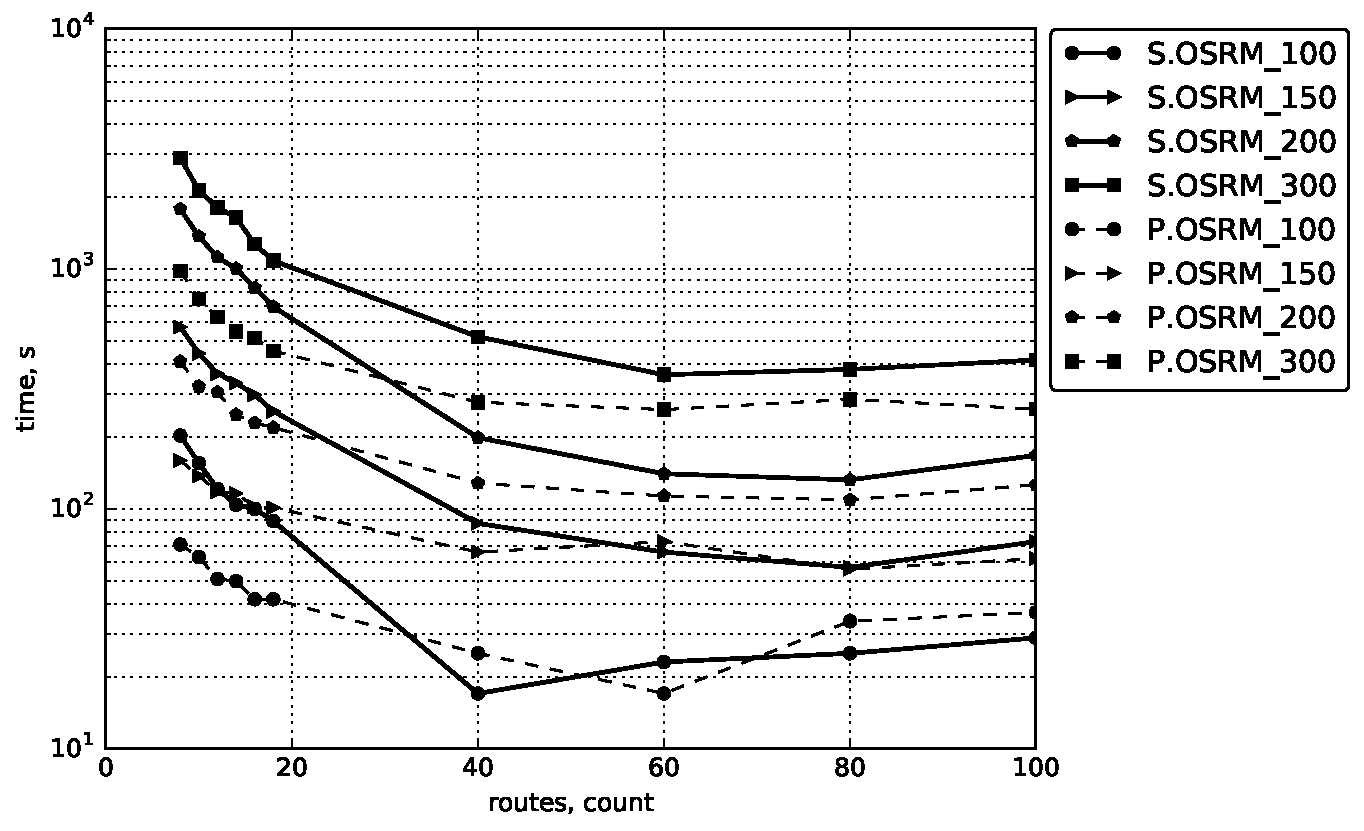
\includegraphics[width=\textwidth]{result-01}
    \caption{Зависимость времени построения от количества маршрутов}
    \label{fig:result-01}
\end{figure}

\begin{figure}[ht!]
    \centering
    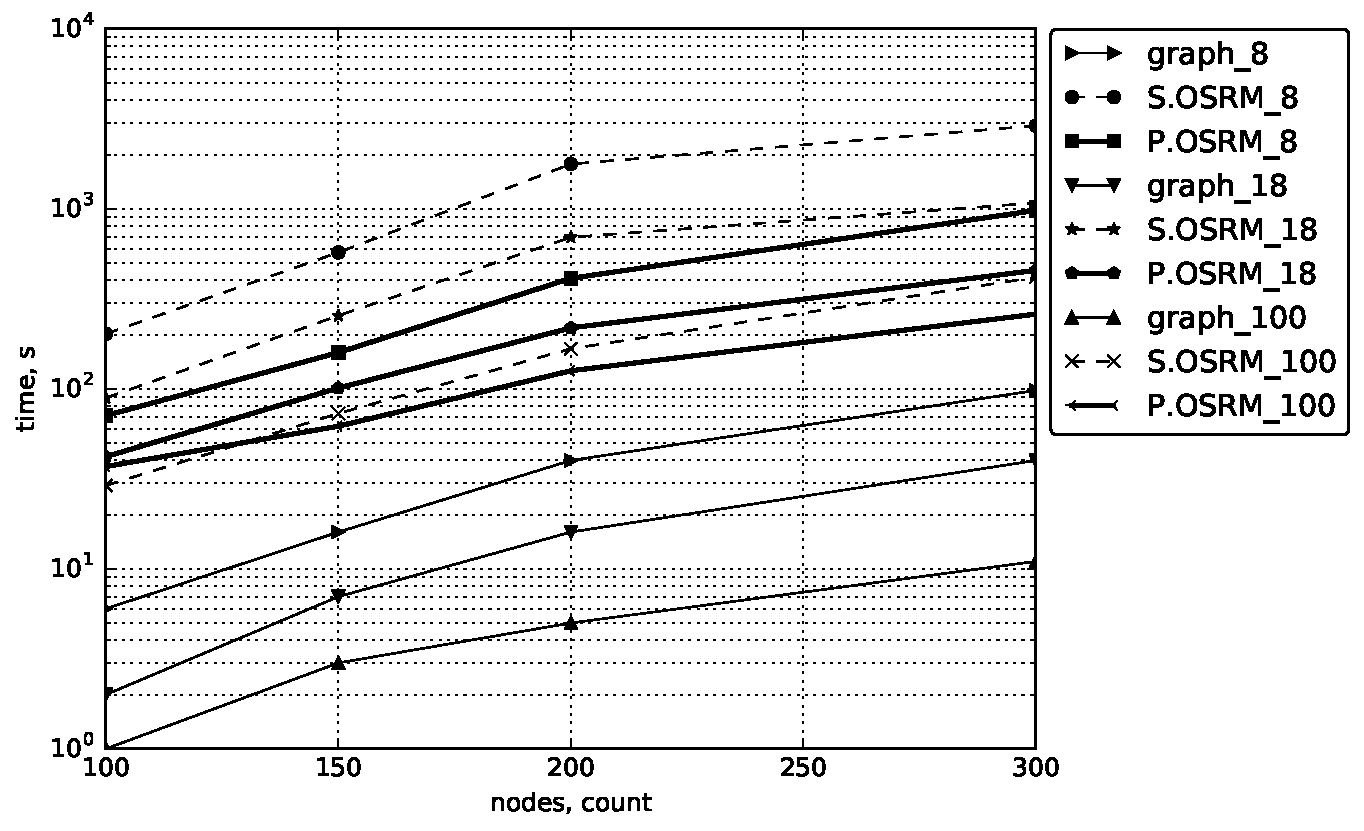
\includegraphics[width=\textwidth]{result-02}
    \caption{Зависимость времени построения от кластеров}
    \label{fig:result-02}
\end{figure}

\begin{figure}[ht!]
    \centering
    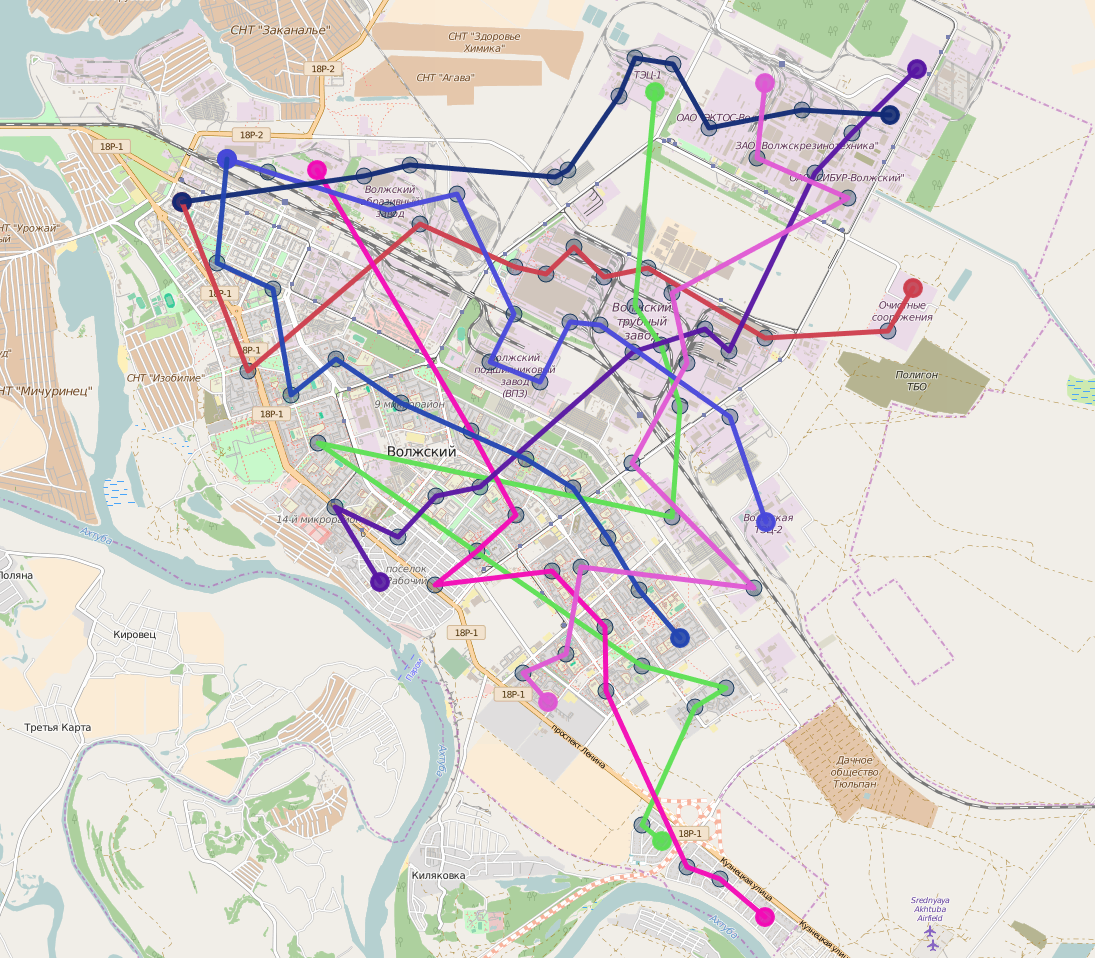
\includegraphics[width=0.8\textwidth]{100-8}
    \caption{Использование метрики graph для 100 кластеров и 8 маршрутов.}
    \label{fig:network-01a}
\end{figure}

\begin{figure}[ht!]
    \centering
    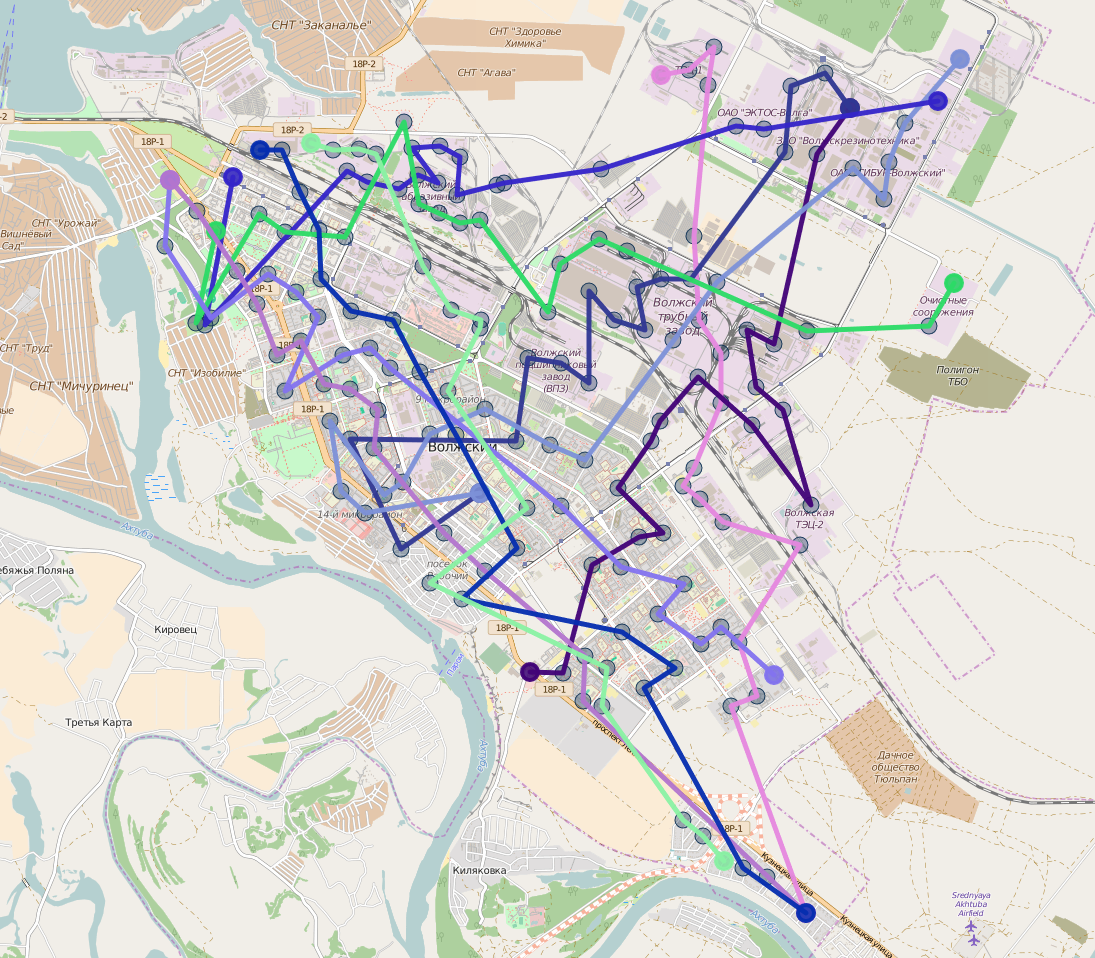
\includegraphics[width=0.8\textwidth]{200-10}
    \caption{Использование метрики graph для 200 кластеров и 10 маршрутов.}
    \label{fig:network-01b}
\end{figure}

\begin{figure}[ht!]
    \centering
    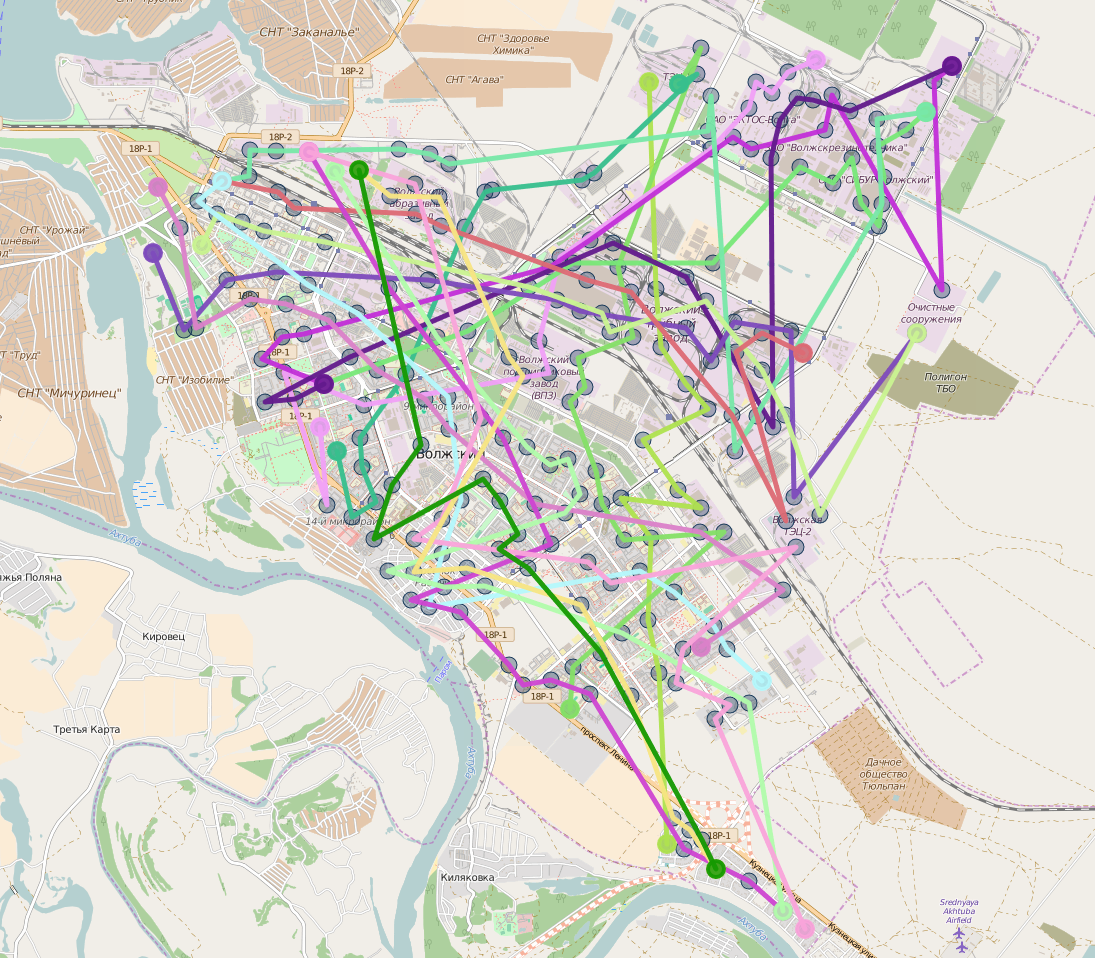
\includegraphics[width=0.8\textwidth]{300-18}
    \caption{Использование метрики graph для 300 кластеров и 18 маршрутов.}
    \label{fig:network-01c}
\end{figure}

\begin{figure}[ht!]
    \centering
    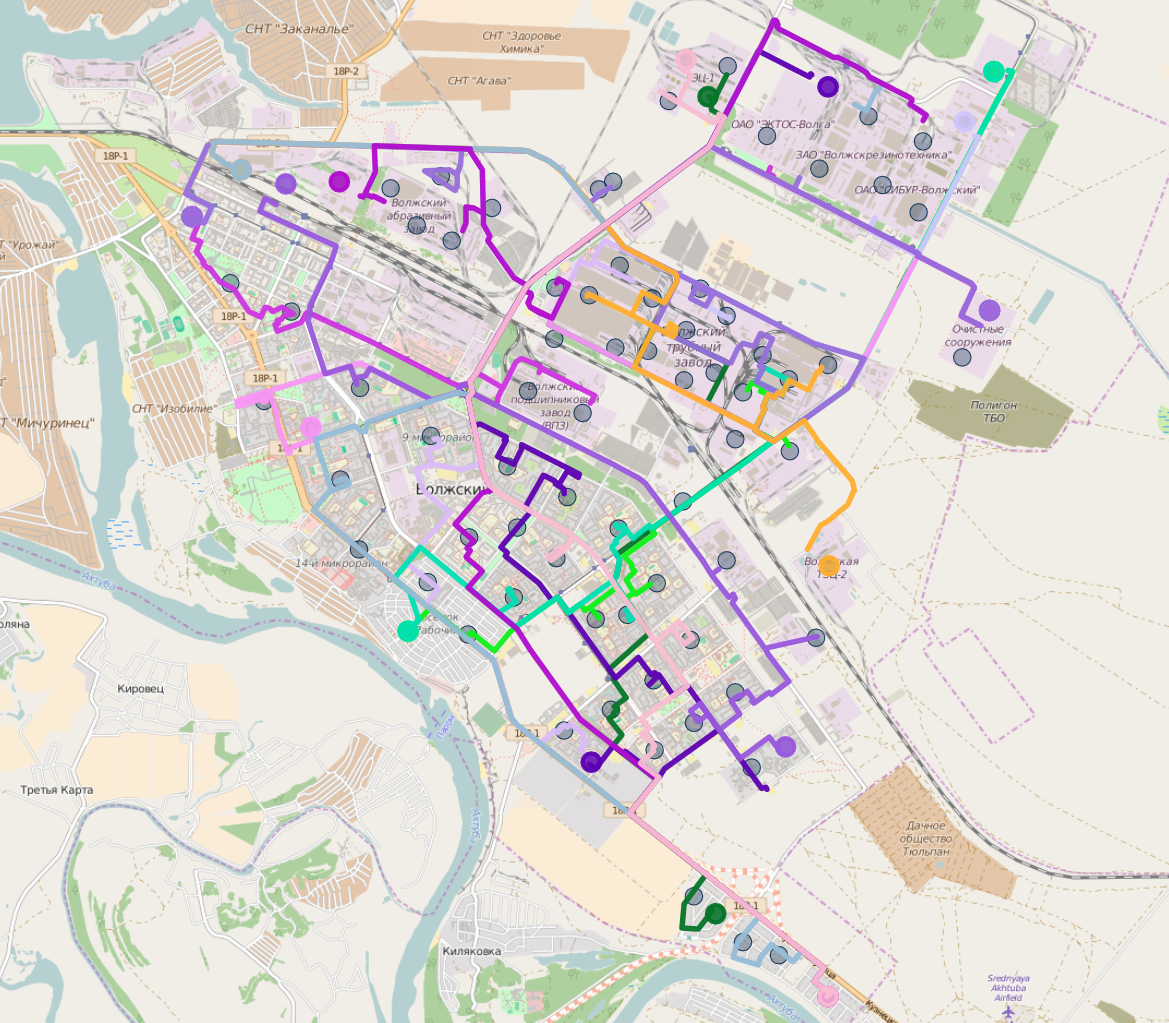
\includegraphics[width=0.8\textwidth]{100-14}
    \caption{Использование метрики OSRM для 100 кластеров и 14 маршрутов.}
    \label{fig:network-02a}
\end{figure}

\begin{figure}[ht!]
    \centering
    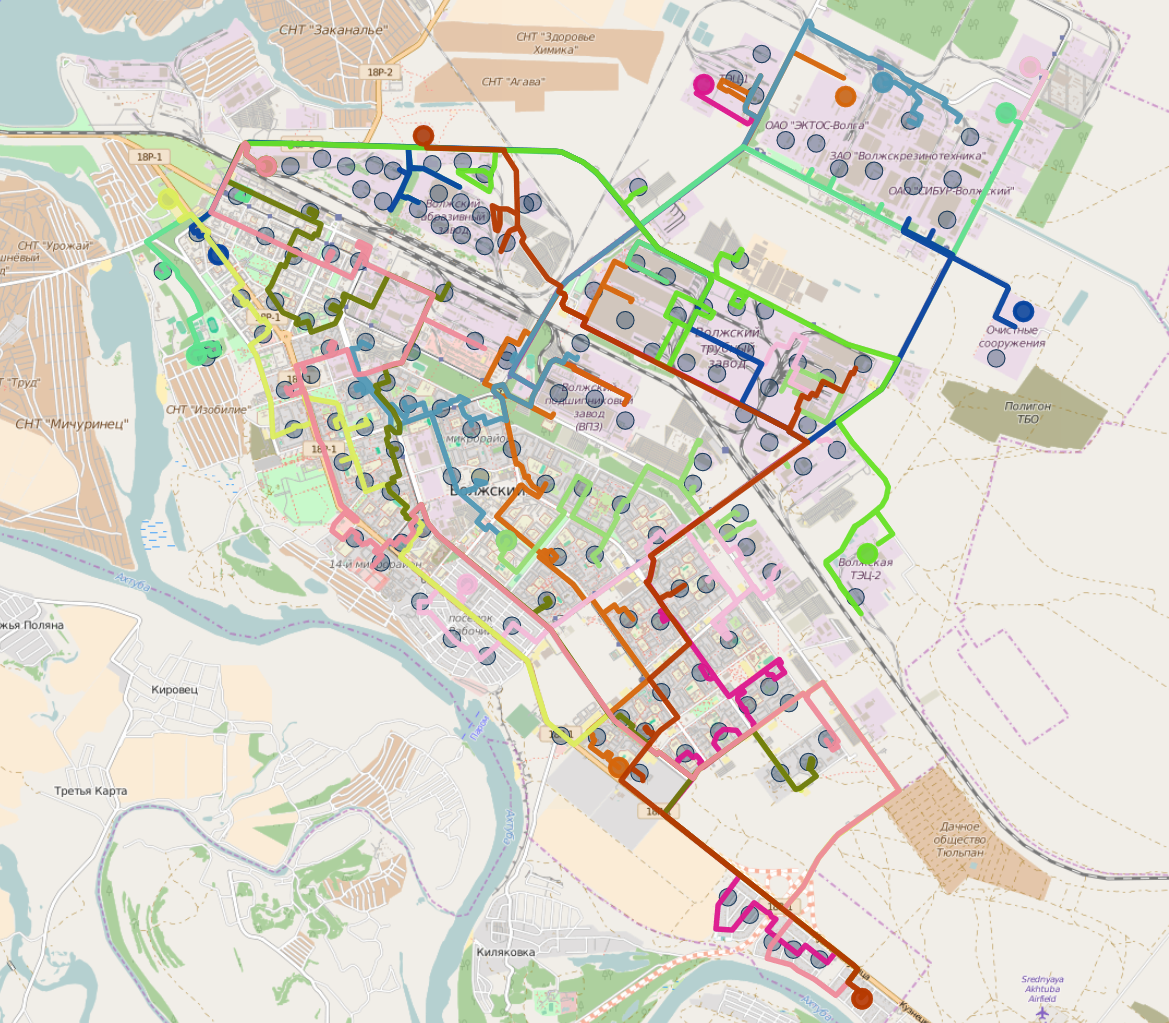
\includegraphics[width=0.8\textwidth]{200-12}
    \caption{Использование метрики OSRM для 200 кластеров и 12 маршрутов.}
    \label{fig:network-02b}
\end{figure}

\clearpage

\begin{figure}[ht!]
    \centering
    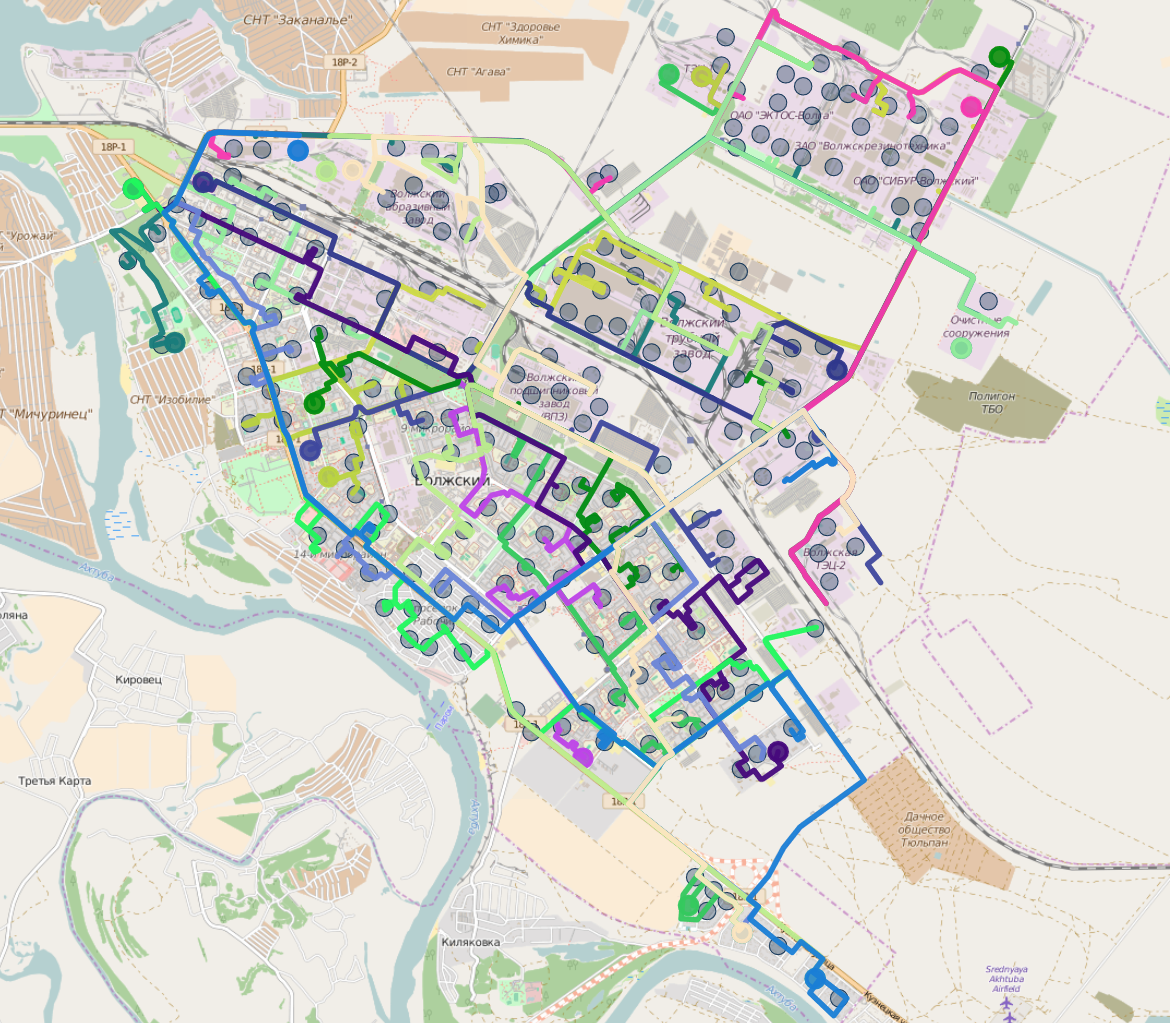
\includegraphics[width=0.8\textwidth]{300-16}
    \caption{Использование метрики OSRM для 300 кластеров и 16 маршрутов.}
    \label{fig:network-02c}
\end{figure}

\begin{table}[ht!]
    \centering
    \caption{Результаты эксперимента алгоритма из пункта \ref{sec:second_alg}.\\
        Данные представлены в формате минуты:секунды.}
    \label{table-time-results}
    \small
    \begin{tabular}{|c|l|c|c|c|c|c|c|l|l|l|c|}
        \hline
        \multicolumn{1}{|l|}{}      &          & \multicolumn{10}{c|}{количество маршрутов}                                                                                                       \\ \hline
        \multicolumn{1}{|l|}{узлы} & стратегия & 8     & 10    & 12    & 14    & 16    & 18    & \multicolumn{1}{c|}{40} & \multicolumn{1}{c|}{60} & \multicolumn{1}{c|}{80} & 100  \\ \hline
        \multirow{3}{*}{100}        & graph    & 0:06  & 0:04  & 0:03  & 0:03  & 0:02  & 0:02  & 0:01                    & 0:01                    & 0:01                    & 0:01 \\ \cline{2-12} 
        & S. OSRM  & 3:22  & 2:35  & 2:01  & 1:44  & 1:40  & 1:29  & 0:17                    & 0:23                    & 0:25                    & 0:29 \\ \cline{2-12} 
        & P. OSRM  & 1:11  & 1:03  & 0:51  & 0:50  & 0:42  & 0:42  & 0:25                    & 0:17                    & 0:34                    & 0:37 \\ \specialrule{.05em}{.02em}{.02em}
        \multirow{3}{*}{150}        & graph    & 0:16  & 0:12  & 0:10  & 0:08  & 0:07  & 0:07  & 0:04                    & 0:03                    & 0:02                    & 0:03 \\ \cline{2-12} 
        & S. OSRM  & 9:32  & 7:24  & 6:06  & 5:34  & 4:59  & 4:15  & 1:27                    & 1:06                    & 0:57                    & 1:13 \\ \cline{2-12} 
        & P. OSRM  & 2:39  & 2:17  & 1:58  & 1:56  & 1:42  & 1:41  & 1:06                    & 1:13                    & 0:56                    & 1:02 \\ \specialrule{.05em}{.02em}{.02em}
        \multirow{3}{*}{200}        & graph    & 0:40  & 0:31  & 0:25  & 0:20  & 0:20  & 0:16  & 0:08                    & 0:06                    & 0:05                    & 0:05 \\ \cline{2-12} 
        & S. OSRM  & 29:33 & 22:45 & 18:36 & 16:43 & 13:53 & 11:35 & 3:18                    & 2:20                    & 2:12                    & 2:47 \\ \cline{2-12} 
        & P. OSRM  & 6:51  & 5:23  & 5:06  & 4:07  & 3:48  & 3:38  & 2:08                    & 1:53                    & 1:49                    & 2:06 \\ \specialrule{.05em}{.02em}{.02em}
        \multirow{3}{*}{300}        & graph    & 1:38  & 1:16  & 1:02  & 0:51  & 0:46  & 0:40  & 0:20                    & 0:14                    & 0:11                    & 0:11 \\ \cline{2-12} 
        & S. OSRM  & 48:20 & 35:24 & 30:00 & 27:17 & 21:06 & 18:01 & 8:41                    & 6:02                    & 6:21                    & 6:57 \\ \cline{2-12} 
        & P. OSRM  & 16:20 & 12:28 & 10:31 & 9:08  & 8:35  & 7:35  & 4:38                    & 4:19                    & 4:46                    & 4:20 \\ \hline
    \end{tabular}
\end{table}

\clearpage

\section{Обсуждение результатов}
На основе результатов алгоритма \ref{alg:min-length} необходимо проанализировать следующее: (I) анализ 
эффективности различных стратегий реализации; (II) как производительность зависит от заранее определенного 
числа узлов в сети; (III) как производительность (с точки зрения сложности времени) зависит от заранее 
определенного количества маршрутов в сети; (IV) общая длина окончательной сети.

Как и ожидалось стратегия 'graph' является самой быстрой по времени вычисления и не требующая сторонних 
сервисов для расчёта. 'S.OSRM' проигрывает стратегии 'P.OSRM' до 3-х раз, и эта зависимость остается 
неизменной независимо от количества узлов в постановки задачи. Заметим, что больше половины времени тратится 
на запросы к сервису OSRM. Это можно рассматривать как узкое место данной программной реализации.

При увеличении количества узлов становится заметно их сильное влияние на производительности алгоритма. Это 
наиболее очевидно для реализации 'S.OSRM'. На основе эмпирической оценки сложности (с точки зрения времени 
расчета), сложность алгоритма может быть оценена как \( O(N^3) \), где \( N \) является числом узлов в 
графе. Но при увеличение числа маршрутов (до определенного значения) начинает уменьшатся время вычисления. 
Это можно объяснить тем тем, что на каждом шагу, необходимо перебрать \( C_{nt} - n_r \) нераспределенных 
узлов, т.е на каждой итерации алгоритма из расчёта исключаются \( n_r \) узлов, что способствует завершить 
работу за меньший промежуток времени на большем количестве маршрутов.

Для визуальной оценки качества построенной маршрутной сети рисунки \ref{fig:network-01a} -- 
\ref{fig:network-01c} представляющие стратегию 'graph' являются более наглядными для анализа, чем рисунки 
представляемые стратегией с использованием сервиса OSRM, но не могут претендовать на роль эффективной 
реализации из-за явного отсутствия учёта естественных и искусственных препятствий. Визуальный анализ 
стратегий с использованием сервиса OSRM затруднён тем, что происходит наложение построенных маршрутов друг 
на друга, да и данные полученные с его помощью не могут быть объективными. Поэтому не будем акцентировать на 
нём своё внимание.

С экономической точки зрения, качество сети маршрутов может быть выражено в терминах длины сети. Согласно 
расчетам, длина сети возрастает пропорционально числу маршрутов. Например, длина сети для 8-ми маршрутов с 
100 узлами -- \( 199\ 532 \) м в сравнении с 18-ти маршрутной сетью -- с \( 305\ 671 \) м с таким же 
количеством узлов. Протяженность сети 8-ми маршрутов с 300 узлами -- \( 335\ 090 \) м в сравнению с 18-ти 
маршрутной сетью -- \( 492\ 583 \) м с таким же количеством узлов. 

Это можно рассматривать как недостаток метода, но объективная оценка должна включать в себя расстояние 
пешего хода, время в пути и ряд других параметров, которые смогут оценить работу алгоритма со всех сторон. 
Но как правило, сеть с несколькими <<длинными>> маршрутами построенная данным алгоритмом является 
неэффективной.

В целом алгоритм является оптимальным, как некоторое приближение, для создания сети маршрутов общественного 
транспорта. Его применение оправдает себя при использовании в связке с другим алгоритмом, для которого 
необходимо иметь начальную конфигурацию транспортной сети.

\section{Заключение}
В данной главе был проанализирован и протестирован алгоритм для построения сети маршрутов основанного на 
обработке геораспределенных данных, а также представлены и объяснены три его реализации и произведена оценка 
производительности данного алгоритма. На основе эвристической оценки алгоритм имеет кубическую временную 
сложность и возможность по взаимодействию с внешними службами (например, OSRM). В результате протестированный 
алгоритм можно использовать для создания предварительной сети маршрутов общественного транспорта или как 
промежуточное звено для создания начальной сети с последующей её модификацией.